\section{Phase 3: Initial Baseline Identification}
In this phase, we aimed to identify the initial emotional baseline of each participant by mapping their emotional data points onto the valence-arousal space. For this purpose, we used the fused emotional data collected in the previous phase. Each participant's emotional expressions were visualized on the two-dimensional plane, representing emotional valence and arousal. The full mapping of all participants' initial emotional data points is shown in Figure~\ref{fig:initial-mappings-grid}.

\begin{figure}[H]
    \centering
    \includegraphics[width=1\textwidth]{img/chapter_04/baseline/participant_initial_mapping.png}
    \caption{Initial Emotional data mapping for all participants}
    \label{fig:initial-mappings-grid}
\end{figure}

To estimate the baseline more accurately, we applied KDE over the mapped points. After identifying the baseline zones using KDE, we evaluated the correctness and reliability of the results through a participant questionnaire. 


\subsection*{Baseline Identification via KDE}
After mapping the emotional data points using KDE, we examined the resulting density distributions to find the regions with the highest concentration of data. For each participant, we generated 3D surface plots showing these density values, as presented in Figure~\ref{fig:kde-3d-plots}. The peak of each surface represents the potential baseline. We selected a 0.1 $\times$ 0.1 area around the point of highest density. This square region was taken as the baseline zone. The exact valence and arousal values at the peak density, along with the top-left and bottom-right coordinates of the baseline square, are presented in Table~\ref{tab:baseline-kde-values}.


\begin{table}[H]
    \centering
    \caption{Participant baseline values estimated from KDE peak density}
    \label{tab:baseline-kde-values}
    \begin{tabular}{|c|c|c|c|c|c|}
        \hline
        \textbf{Participant} & \textbf{Valence} & \textbf{Arousal} & \textbf{Max Density} & \textbf{Top-Left } & \textbf{Bottom-Right} \\
        \hline
        p1  & 0.20  & -0.07 & 597.3728 & (0.15, -0.02) & (0.25, -0.12) \\
        p2  & -0.04 & -0.15 & 690.2971 & (-0.09, -0.10) & (0.01, -0.20) \\
        p3  & 0.21  & -0.07 & 337.2014 & (0.16, -0.02) & (0.26, -0.12) \\
        p4  & 0.05  & 0.01  & 430.7903 & (0.00, 0.06) & (0.10, -0.04) \\
        p5  & 0.17  & -0.18 & 366.9585 & (0.12, -0.13) & (0.22, -0.23) \\
        p6  & -0.16 & -0.09 & 489.9168 & (-0.21, -0.04) & (-0.11, -0.14) \\
        p7  & -0.16 & -0.10 & 345.6209 & (-0.21, -0.05) & (-0.11, -0.15) \\
        p8  & -0.22 & -0.06 & 262.2035 & (-0.27, -0.01) & (-0.17, -0.11) \\
        p9  & -0.12 & 0.09  & 335.896  & (-0.17, 0.14) & (-0.07, 0.04) \\
        p10 & 0.19  & 0.01  & 318.8352 & (0.14, 0.06) & (0.24, -0.04) \\
        \hline
    \end{tabular}
\end{table}


The identified baseline zones were also visualized on a 2D plane for better interpretability, as shown in Figure~\ref{fig:kde-2d-baselines}. This visual comparison allows us to see how each participant's baseline position varies in the valence-arousal space.

\begin{figure}[H]
    \centering
    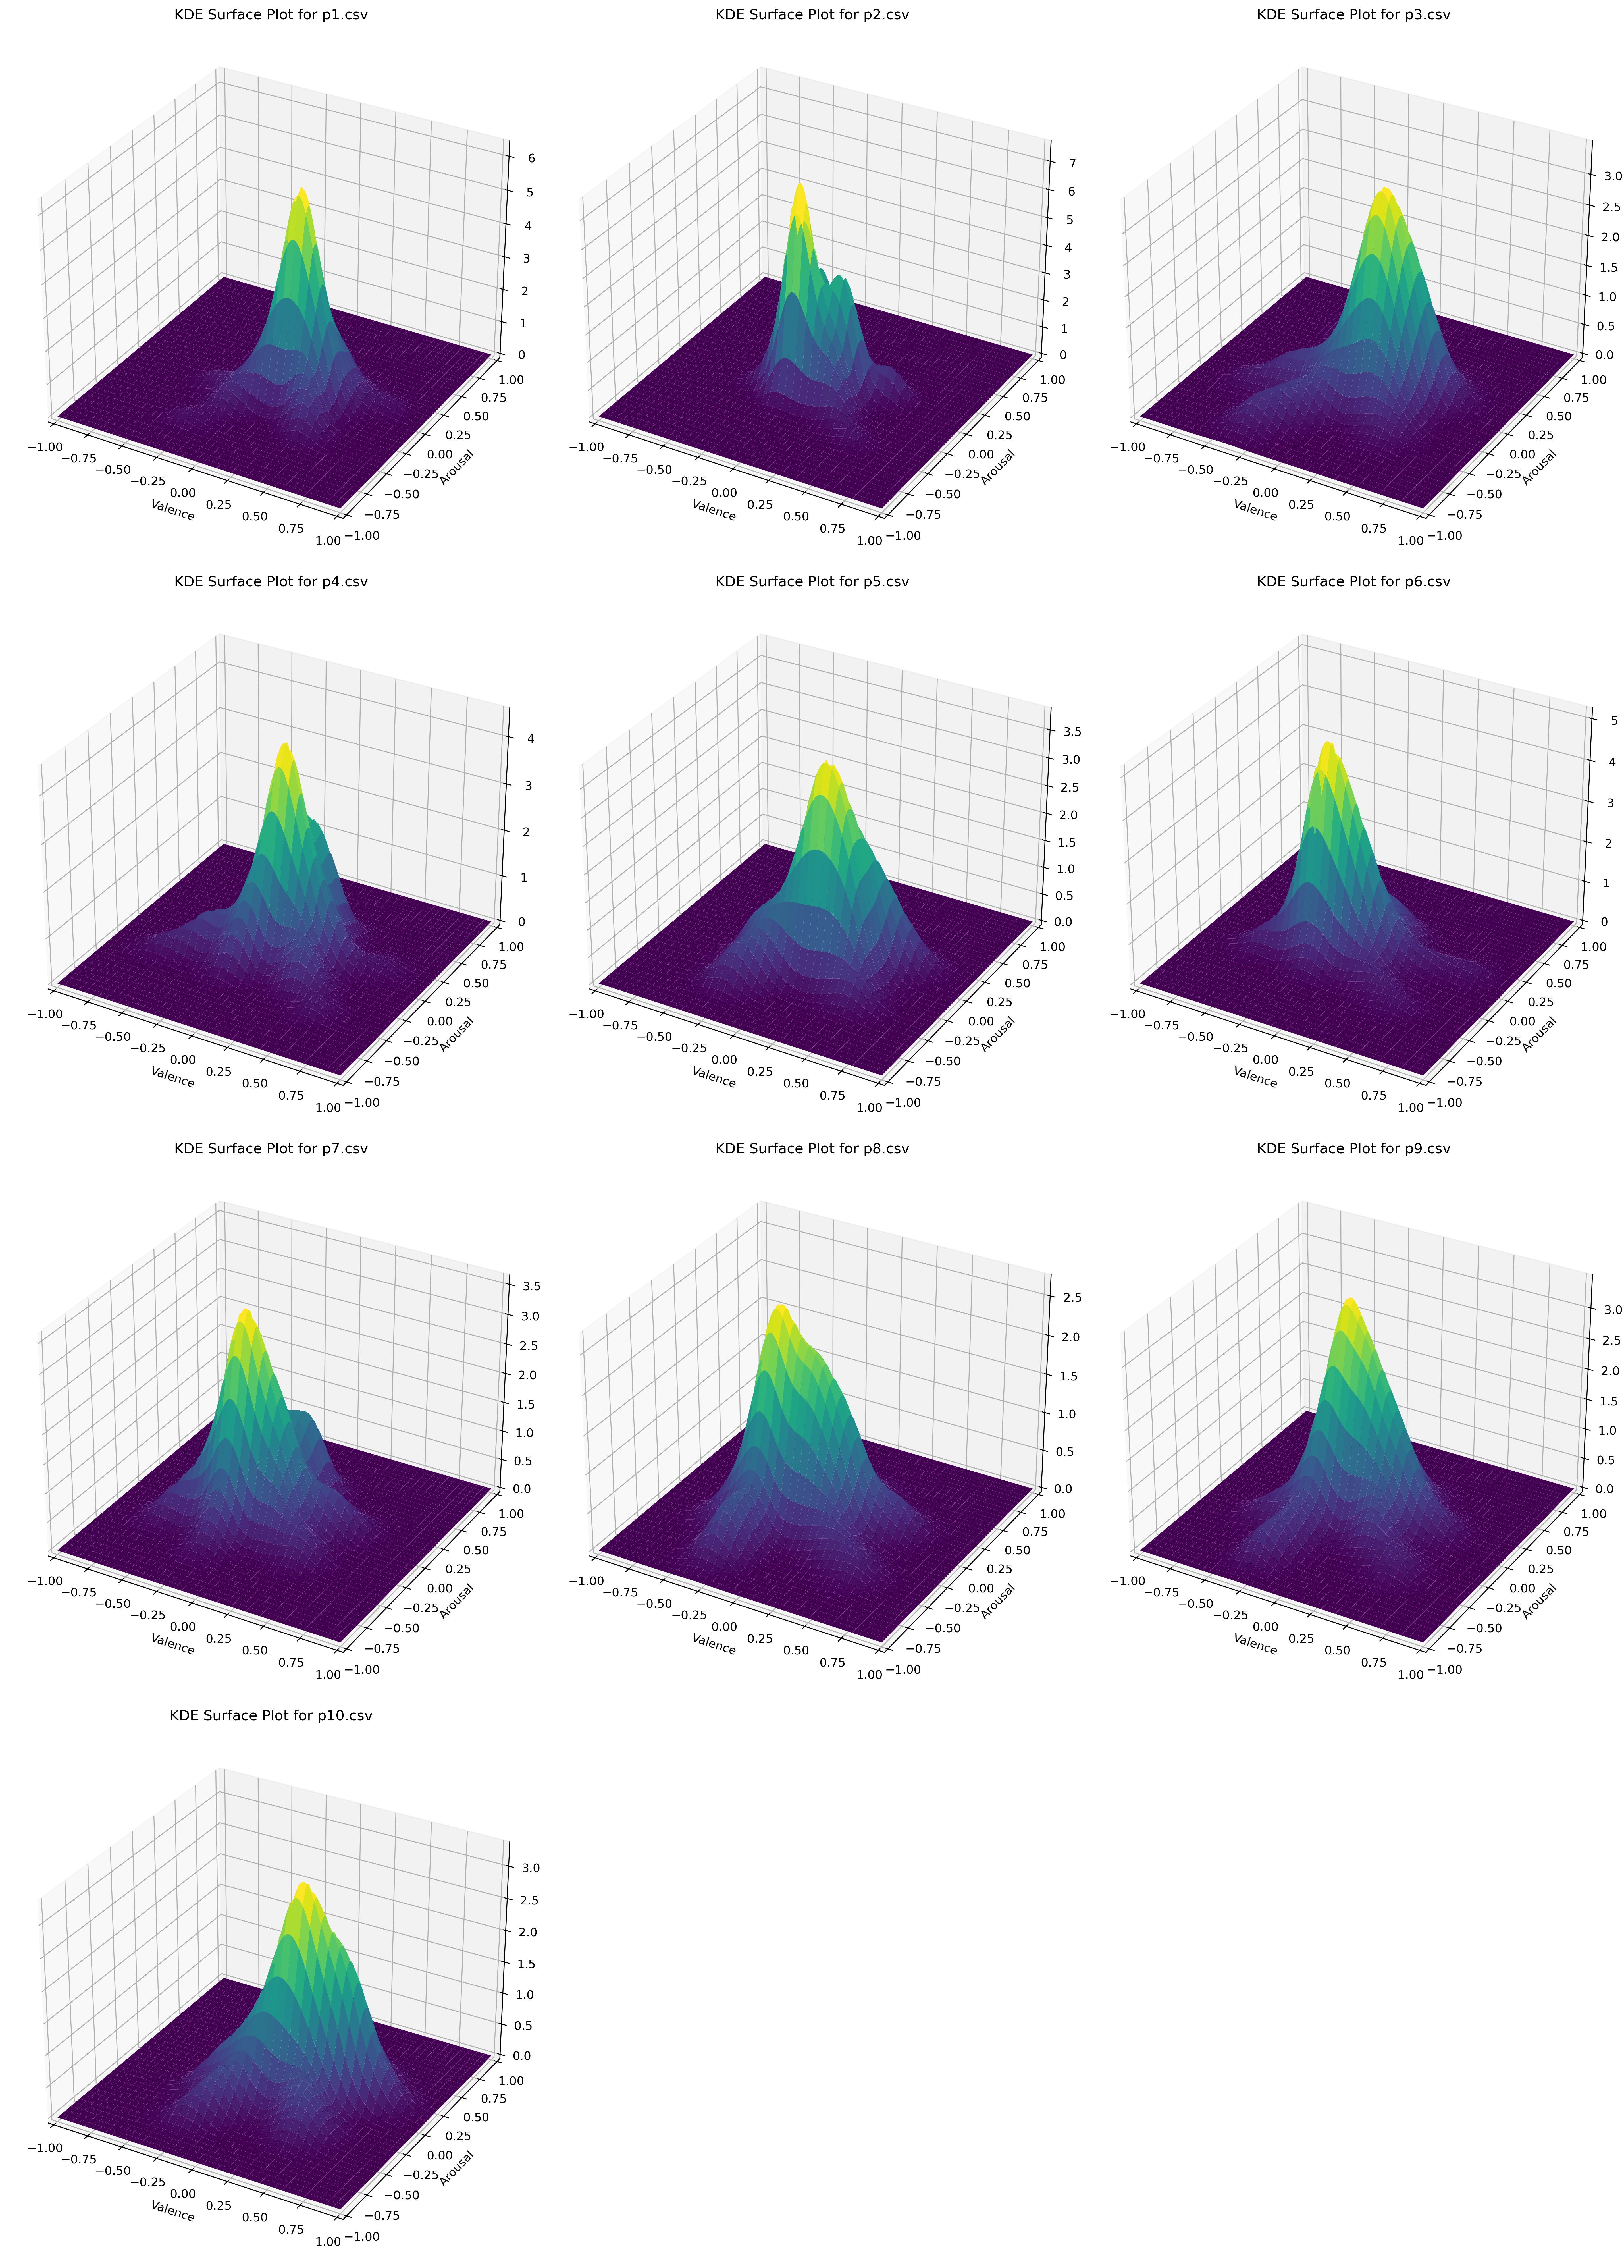
\includegraphics[width=0.80\textwidth]{img/chapter_04/baseline/kde_surface_all-new.png}
    \caption{3D surface plots of KDE-based emotional distributions for all participants}
    \label{fig:kde-3d-plots}
\end{figure}


\begin{figure}[H]
    \centering
    \includegraphics[width=0.80\textwidth]{img/chapter_04/baseline/kde_2d_baseline_map-new.png}
    \caption{2D mapping of KDE-estimated baseline zones for each participant}
    \label{fig:kde-2d-baselines}
\end{figure}


\subsection*{Evaluation}

To evaluate the accuracy and relevance of the identified baseline values, we conducted a questionnaire with all participants. Each participant was asked to reflect on the emotional states represented in their baseline region and indicate how closely those states matched their typical emotional condition during the experiment sessions.

The full questionnaire and participant responses are provided in the Appendix (see Section~\ref{sec:appendix-questionnaire}). Based on the collected responses, we calculated the frequency of agreement between the participants and the computed baseline zones. This frequency distribution is shown in Figure~\ref{fig:baseline-agreement-bar}, which highlights the overall agreement levels across all participants.

In addition, we visualized the relationship between the identified baselines and the participants’ self-reported emotional states using a valence-arousal scatter plot. This comparison, presented in Figure~\ref{fig:baseline-scatter-plot}, helps illustrate how closely the KDE-based baseline aligns with the participants' own perception.

\begin{figure}[H]
    \centering
    \includegraphics[width=0.75\textwidth]{img/chapter_04/baseline/agreement_bar.png}
    \caption{Participant agreement frequency with identified baseline values}
    \label{fig:baseline-agreement-bar}
\end{figure}

\begin{figure}[h]
    \centering
    \includegraphics[width=1\textwidth]{img/chapter_04/baseline/valence_arousal_scatter.png}
    \caption{Scatter plot comparing identified and participant-proposed baseline coordinates}
    \label{fig:baseline-scatter-plot}
\end{figure}


The analysis of the questionnaire responses provides valuable insights into the accuracy and acceptance of the computed baseline values. 

\textbf{General Agreement Level:} The mean agreement score for Question 1  was 3.70 out of 5, indicating that most participants tended to agree with their computed emotional baseline. Furthermore, 60\% of participants explicitly expressed agreement, which supports the reliability of the baseline computation method for the majority.

\textbf{Baseline Discrepancy:} To measure how much the participants’ proposed baselines differed from the computed values, we used the Euclidean distance.
The mean distance was found to be 0.120 with a standard deviation of 0.122. This result shows that, on average, participants' self-identified baseline points differ from the computed values by around 0.12 units in the valence-arousal space. The similarity between the mean and standard deviation also indicates a consistent pattern in how much the computed and proposed baselines deviate from each other. Table~\ref{tab:agreement_summary} summarizes the computed distances for each participant.

\begin{table}[H]
    \centering
    \caption{Participant Agreement and Baseline Discrepancy Summary}
    \begin{tabular}{lcccc}
    \toprule
    \textbf{Participant ID} & \textbf{Agreement (1-5)} & \textbf{Proposed (Valence, Arousal)} & \textbf{Distance} \\
    \midrule
    P1 & 4 & (0.25, -0.05) & 0.054 \\
    P2 & 3 & (0.40, -0.02) & 0.230 \\
    P3 & 4 & (0.20, 0.10) & 0.305 \\
    P4 & 5 & (0.23, -0.06) & 0.014 \\
    P5 & 3 & (-0.05, 0.15) & 0.071 \\
    P6 & 4 & (0.35, -0.10) & 0.054 \\
    P7 & 2 & (0.20, 0.20) & 0.321 \\
    P8 & 4 & (0.24, -0.07) & 0.014 \\
    P9 & 3 & (0.10, -0.05) & 0.134 \\
    P10 & 5 & (0.21, -0.10) & 0.000 \\
    \bottomrule
    \end{tabular}
    \label{tab:agreement_summary}
    \end{table}
    